% state-of-the-art_patent.tex
%
% Drafted by Juntang on August 21, 2024
% ReDragted by Juntang on August 22, 2024

\begin{frame}
  \frametitle{State of the Art (I)}
  \cite{Dt_patent_wo2005104936a12005}
    \begin{columns}
    %% double-column layout 
    \begin{column}{0.45\textwidth}                 %% Left Column
    {\small
    \begin{enumerate}
        \item $C_{AIF} \rightarrow C_{in}$, assuming $\alpha_1 = 0$:
        \begin{equation}
            C_{in}(t) = \left( C_{AIF} * R_{1}^{[P]} \right)(t)
        \end{equation}
        \begin{equation}
            R_{1}^{[P]}(t) = \left\{
            \begin{array}{ll}
            \frac{1}{\sigma_1} e^{-\frac{t - AT_1}{\sigma_1}}, & \text{if } t \geq AT_1 \\
            0, & \text{otherwise}
            \end{array}\right.
        \end{equation}
        %
        \item $C_{in} \rightarrow C_{tissue}$, assuming $AT_2 = 0$:
        \begin{equation}
        C_{tissue}(t) = \frac{Q}{k_H}\left( C_{in} * R_{2}^{[P]} \right)(t)
        \end{equation}
        \begin{equation}
            R_{2}^{[P]}(t) = 1 - \int_0^t \frac{\tau^{\alpha_2}}{\Gamma(1 + \alpha_2) \sigma_2^{1+\alpha_2}} e^{-\frac{\tau}{\sigma_2}} d\tau 
        \end{equation}
    \end{enumerate}
    }
    \end{column}
    
    \hspace*{4em}                                                          %%  make space between columns 
    
    \begin{column}{0.42\textwidth}                 %% Right Column 
        \begin{figure}
            \centering
            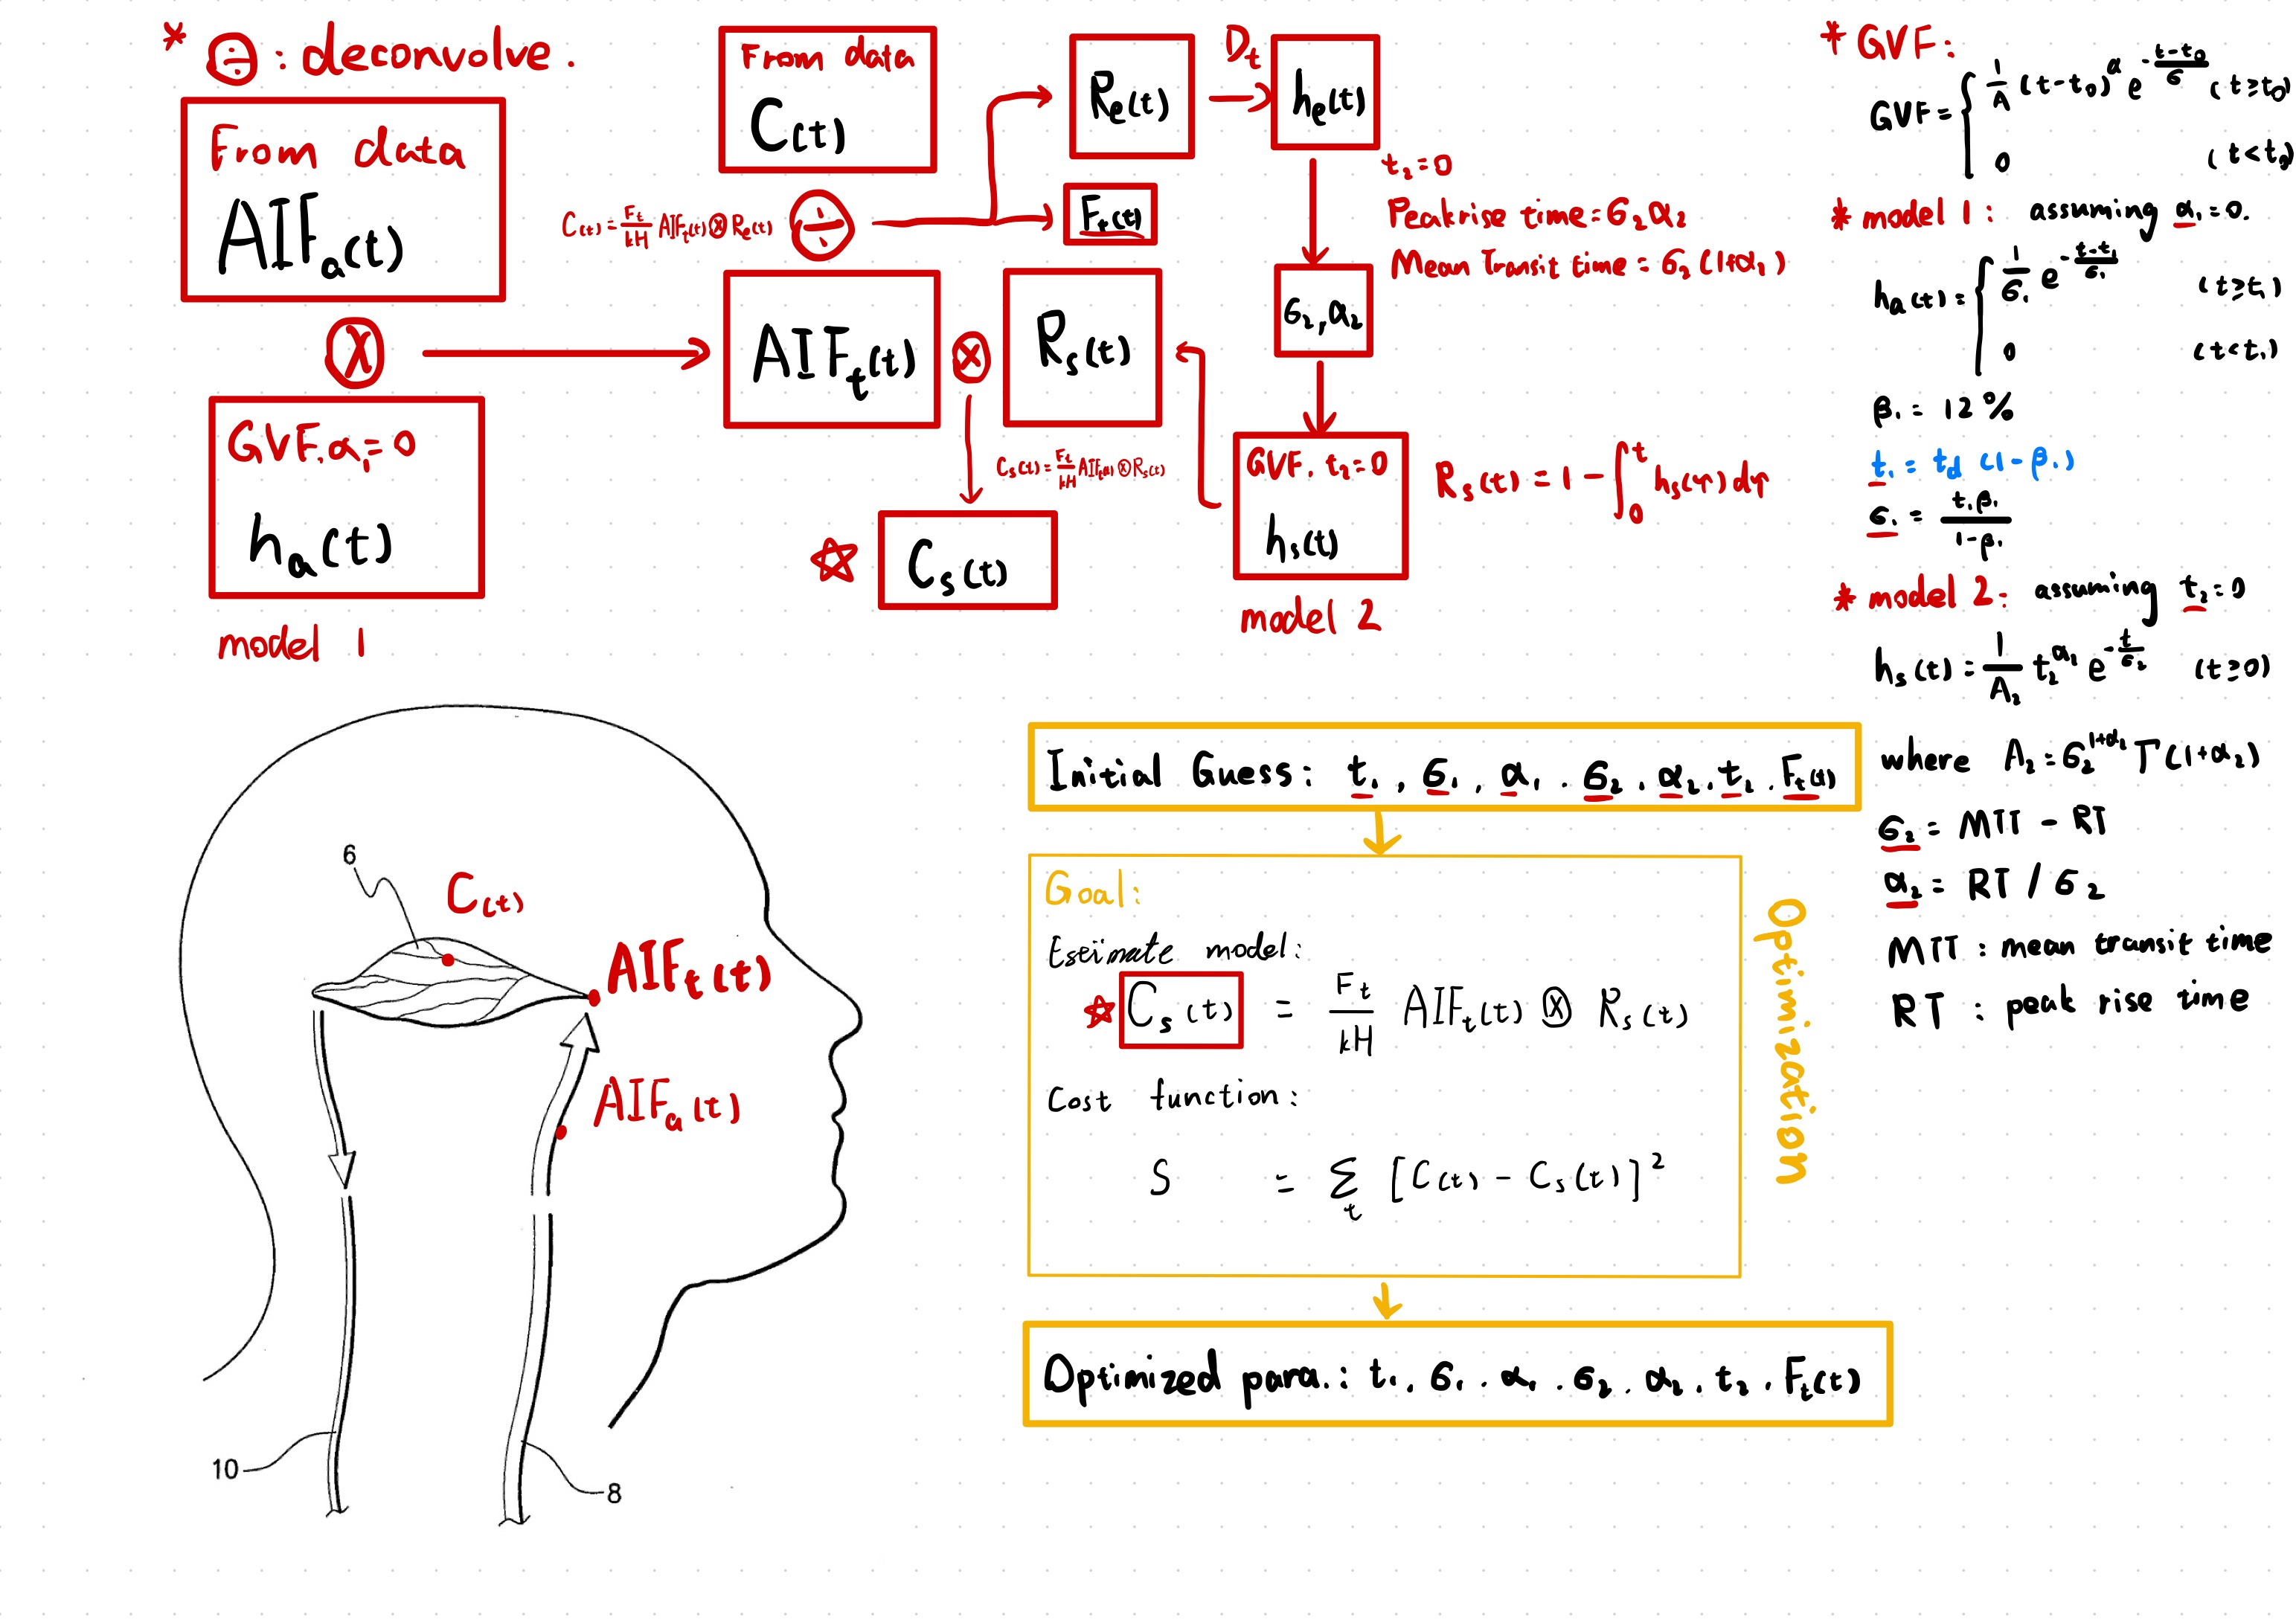
\includegraphics[width=\linewidth]{figures/intro-patent.jpg}
            \caption{Flowchart summarizing the methodology of \cite{Dt_patent_wo2005104936a12005}}
            \label{fig:patent}
        \end{figure}
    \end{column}
    %
    \end{columns}   %% End of multiple columns 
    % 

\end{frame}

%%% Local Variables:
%%% mode: latex
%%% TeX-master: "../topic-slide-main"
%%% End: